% Chapter Template

\chapter{Synchronization-free and always-synchronizing LTNs}

\section{Synchronization-free negotiations}
\label{sec:synchr-free-negot}

Our goal is to study the location reachability problem in local-timed
negotiations. Before studying the general case, we look at some
restricted versions. The first restriction we look at is a
synchronization-free fragment. Fix a negotiation
$\Nn = (N, \dom, \delta, \Sync)$ for this section.

We say that $\Nn$ is \emph{synchronization-free} if
$\Sync = \emptyset$. In such a negotiation, the agents require to
elapse sufficient time only to satisfy their local guards (and not to
meet any synchronization criteria). For instance, in the example on
the left of Figure~\ref{fig:k-vendor}, if $n_3$ is not a synchronizing
node, then $q$ can come directly to $n_3$ after node $n_1$, elapse no
time at all, and engage in the only outcome from $n_3$. In the
negotiation of Figure~\ref{fig:abc}, if the outcome $c$ is not
synchronized, the untimed language is the set of $wc$ where
$w \in (a + b)^*$ contains at least one $a$ and one $b$.

Although the time elapse needed for an agent is to satisfy her own
guards, she may need to collaborate with a partner to decide on what
amount to elapse. This is because of the combination of guards across
the different agents at a location. This is apparent in the
negotiation of Figure~\ref{fig:nonsync}. For $c$ to be feasible, both
the agents have to reach node $n_4$ via $n_2$, and not via
$n_3$. Therefore, one can view the time elapse at $n_1$ as a
collective decision between $p$ and $q$, which impacts their future
paths.

\begin{figure}[t]
\centering 
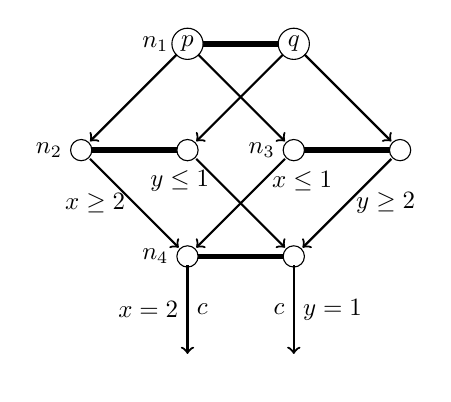
\begin{tikzpicture}[scale=0.9, every node/.style={transform shape}]

\begin{scope}[line width=2pt]
\draw (0,0) node [left] {$n_1\,\,$} -- (1.5,0);
\draw (-1.5,-1.5) node [left] {$n_2\,\,$} -- (0,-1.5);
\draw (1.5,-1.5) node [left] {$n_3\,\,$} -- (3,-1.5);
\draw (0,-3) node [left] {$n_4\,\,$} -- (1.5,-3);
\end{scope}

\filldraw [fill=white]  (0,0)  circle (2.2mm) node 		(n1p) {$p$};
\filldraw [fill=white]  (1.5,0)  circle (2.2mm) node 		(n1q) {$q$};

\filldraw [fill=white]  (-1.5,-1.5)  circle (1.5mm) node 	(n2p) {};
\filldraw [fill=white]  (0,-1.5)  circle (1.5mm) node 	(n2q) {};

\filldraw [fill=white]  (1.5,-1.5)  circle (1.5mm) node 	(n3p) {};
\filldraw [fill=white]  (3,-1.5)  circle (1.5mm) node 	(n3q) {};

\filldraw [fill=white]  (0,-3)  circle (1.5mm) node 		(n4p) {};
\filldraw [fill=white]  (1.5,-3)  circle (1.5mm) node 	(n4q) {};

\filldraw [white, fill=white]  (0,-4.5)  circle (1.5mm) node 	(vp) {};
\filldraw [white, fill=white]  (1.5,-4.5)  circle (1.5mm) node 	(vq) {};

\begin{scope}[thick,->]

\draw (n1p) + (-0.15,-0.15) -- (n2p);
\draw (n1q) + (-0.15,-0.15) -- (n2q);

\draw (n1p) + (0.15,-0.15) -- (n3p);
\draw (n1q) + (0.15,-0.15) -- (n3q);

\draw (n2p) -- (n4p) node [midway, left] {$x \geq 2$};
\draw (n2q) -- (n4q) node [near start, left] {$y \leq 1$};

\draw (n3p) -- (n4p) node [near start, right] {$x \leq 1$};
\draw (n3q) -- (n4q) node [midway, right] {$y \geq 2$};

\draw (n4p) -- (vp) node [midway, right] {$c$} node [midway, left] {$x = 2$};
\draw (n4q) -- (vq) node [midway, left] {$c$} node [midway, right] {$y = 1$};
\end{scope}

\end{tikzpicture}
\caption{Example of a synchronization-free local-timed
    negotiation. If $n_3$ is fired then the guard $y = 1$ on the
    transition from $n_4$ can not be satisfied.}
\label{fig:nonsync}
\end{figure}

The goal of this section is to show that reachability is
\PSPACE-complete for synchronization-free negotiations. Here is an
overview of our proof. Firstly, as there are no synchronization
constraints, we observe that the reference clocks are not useful at
all in this fragment. We will then quotient the space of valuations by
applying the classical region equivalence between clocks of each
agent. This generates a finite automaton that accepts all the untimed
location sequences that are feasible in the negotiation.

\begin{definition}[$\equiv^p_M$ and $\reg$ equivalences]
  Let $p$ be an agent, and let $M$ be the biggest constant appearing
  in the negotiation. We say $v \preg v'$ if for all $x, y \in X_p$:
  \begin{itemize}
  \item either $\int{v(x)} = \int{v'(x)}$ or both
    $\int{v(x)}, \int{v'(x)} > M$,
  \item if $v(x) \le M$, then $\frac{v(x)} = 0$ iff $\frac{v'(x)} = 0$
    
  \item if $v(x) \le M$ and $v(y) \le M$, we have
    $\frac{v(x)} \le \frac{v(y)}$ iff $\frac{v'(x)} \le \frac{v'(y)}$.
  \end{itemize}
  We define $v \reg v'$ if $v \preg v'$ for all agents $p \in P$. We
  denote by $\region{v}$ the equivalence class of a valuation $v$ with
  respect to the $\reg$ equivalence. We will call $\reg$ as the
  \emph{product-region} equivalence, and the equivalence classes of
  $\reg$ as product-regions.
\end{definition}

Notice that reference clocks do not appear at all in the above
definition. We next state there are finitely many product-regions.

\begin{lemma}\label{lem:size-of-product-regions}
The $\reg$ equivalence is of finite index: the number of
product-regions is bounded by $\Oo(|X|! \cdot 2^{|X|} \cdot
(2M + 1)^{|X|})$.
\end{lemma}


Here are some properties of the product-region equivalence, that
follow from the region equivalence.



\begin{restatable}{lemma}{localDelay}
\label{lemma:region-local-delay}
  Let $v, v'$ be valuations such that $v \reg v'$. Then, for all
  local-delays $\Delta$, there exists a local-delay $\Delta'$ such
  that $v + \Delta \reg v' + \Delta'$.
\end{restatable}


The next lemma follows by definition.
\begin{lemma}\label{lem:region-guard-reset}
  Let $v, v'$ be valuations such that $v \reg v'$. Let $g$ be a guard
  with constants at most $M$. Then: (1) $v \models g$ iff
  $v' \models g$, and (2) for all subsets of local clocks $Y$, we have
  $v[Y] \reg v'[Y]$.
\end{lemma}

For a valuation $v$ and a product-region $r$, we write $v \in r$ to
mean that $r$ equals $[v]$. We will now build a finite automaton using
the product-regions. 


\begin{definition}[Product-region automaton]\label{def:prod-reg-aut}
  States of this NFA are of the form $(C, r)$ where $C$ is a marking
  and $r$ is a product-region. There is a transition
  $(C, r) \xra{(n, a)} (C', r')$ if for some valuation $v \in r$, and
  for some local-delay $\Delta$, we have
  $(C, v) \xra{\Delta, (n, a)} (C', v')$ such that $v' \in r'$. The
  initial state is the initial marking $C_0$ and the region $r_0$
  containing the valuation that maps all clocks to $0$.

  We denote the product-region automaton as $\prg(\Nn)$.
\end{definition}

\begin{lemma}\label{lem:reg-prod-reg-equiv}
  For every run
  $(C_0, v_0) \xra{\Delta_0, \ell_0} (C_1, v_1) \xra{\Delta_1, \ell_1}
  \cdots \xra{\Delta_{m-1}, \ell_{m-1}} (C_m, v_m)$ in the local-timed
  negotiation $\Nn$, there is a run
  $(C_0, [v_0]) \xra{\ell_0} (C_1, [v_1]) \xra{\ell_1} \cdots
  \xra{\ell_{m-1}} (C_m, [v_m])$ in $\prg(\Nn)$. 

  Conversely, for every run
  $(C_0, r_0) \xra{\ell_0} (C_1, r_1) \xra{\ell_1} \cdots
  \xra{\ell_{m-1}} (C_m, r_m)$ in the product-region automaton
  $\prg(\Nn)$, there is a run
  $(C_0, v_0) \xra{\Delta_0, \ell_0} (C_1, v_1)$
  $\xra{\Delta_1, \ell_1} \cdots \xra{\Delta_{m-1}, \ell_{m-1}} (C_m,
  v_m)$ in $\Nn$ such that $v_i \in r_i$ for each $0 \le i \le m$.
\end{lemma}


\begin{theorem}
  Location reachability is \PSPACE-complete for synchronization-free
  local-timed negotiations.
\end{theorem}
\begin{proof}
  A location $\ell = (n,a)$ is reachable in $\Nn$ iff it is reachable
  in $\prg(\Nn)$, thanks to Lemma~\ref{lem:reg-prod-reg-equiv}. Let
  $K$ be the size of the negotiation counted 
  as the sum of the number of nodes, outcomes, clocks and the sum of
  the binary encoding of each constant appearing in the guards. Both the number of markings and the number of
  product-regions is $2^{\Oo(K)}$
  (Lemma~\ref{lem:size-of-product-regions}). Hence the size of the
  product-region graph is $2^{\Oo(K)}$. From the fact that
  $st$-connectivity is in \textsf{LOGSPACE}~\cite{SAVITCH1970177}, we get the \PSPACE\
  upper bound for our problem. 



  \PSPACE-hardness follows from the hardness of timed automata
  reachability~\cite{DBLP:journals/tcs/AlurD94}. Each timed automaton can be seen as a negotiation involving
  a single agent 
  (with 
  a single agent, both notions of local-time and global-time
  coincide). \qed 
\end{proof}

\section{Always-synchronizing negotiations}
\label{sec:always-synchr-negot}

We will now look at the fragment where every interaction forces a
synchronization.  We say that a local-timed negotiation is
\emph{always-synchronizing} if every node is a synchronization node,
that is $\Sync = N$. The negotiation in Figure~\ref{fig:abc} can be
seen as an always-synchronizing negotiation (in nodes that are local
to one agent, the synchronization condition is vacuously true). We
first remark that a region based argument is not immediate in this
fragment. In order to satisfy the synchronization constraint, we check
conditions of the form $t_p = t_q$. Therefore, we cannot decouple the
time elapse of $p$ and $q$ completely, as in the previous
section. Instead, we need to keep track of the difference $t_p - t_q$
in the equivalence. But then, there is no bound $M'$ that allows us to
club together all valuations with $t_p - t_q > M'$. This is because,
$t_q$ can perform local delays to catch up with $p$, and in
particular, from $t_p - t_q > M'$ we may get to a situation where
$t_p - t_q \le M'$. This kind of a mechanics does not happen in
classical timed automata, where once a clock is beyond $M$ it always
stays beyond $M$ until the next reset. In the previous section, we
avoided this problem since we did not need to keep track of the
reference clocks.


We will make use of a different argument altogether, which is used in
the proof of equivalence between the local-time and global-time
semantics for networks of timed
automata~\cite{DBLP:conf/concur/BengtssonJLY98,DBLP:conf/concur/GovindHSW19}. In
always-synchronizing negotiations, every location $(n, a)$ is executed
at a unique timestamp given by the reference clock value of the
participating processes. For example, the sequence $aabbc$ in the
negotiation of Figure~\ref{fig:abc} can be associated with the
timestamp $12123$: the first $a$ occurs at $t_p = 1$, the second $a$
at $t_p = 2$, the first $b$ at $t_q = 1$ and the $c$
occurs when both $t_p = t_q = 3$.  The main
observation is that whenever there is a $t_i t_{i+1}$ in this sequence
with $t_{i+1} < t_i$, we can reorder the actions corresponding to
them, and still get a valid run. For example, the run
$(a, 1) (a, 2) (b, 1) (b, 2) (c, 3)$ described above can be reordered
as $(a, 1) (b, 1) (a, 2) (b, 2) (c, 3)$ which is still a feasible run
of the negotiation.

We will first show that every run of an always-synchronizing sequence
can be reordered to a ``monotonic'' run. Next, we describe a timed
automaton that accepts all monotonic runs of the negotiation. This
gives a procedure for reachability, as reachability in the negotiation
reduces to checking whether there is a run of a timed automaton that
fires an edge.

\begin{definition}
  Let $\Nn$ be an always-synchronizing negotiation. Consider a run
  $\rho:= (C_0, v_0) \xra{\Delta_0, \ell_0} (C_1, v_1) \xra{\Delta_1,
    \ell_1} \cdots \xra{\Delta_{m-1}, \ell_{m-1}} (C_m, v_m)$, where
  $\ell_i = (n_i, a_i)$ for every $i$.

  We associate timestamps $\theta^\rho_i := v_i(t_p) + \Delta_i(p)$
  where $p$ is some agent participating in the negotiation $n_i$.  The
  run $\rho$ is monotonic if $\theta^\rho_i \le \theta^\rho_j$ for
  every $i \le j$.
\end{definition}

Fix an always-synchronizing negotiation $\Nn$ for the rest of this
section.

\begin{restatable}{lemma}{monotonic}
\label{lem:monotonic}
  For every location $(n,a)$ that is reachable, there is a monotonic
  run containing a small step that executes $(n,a)$.
\end{restatable}


\begin{definition}
  For an always-synchronizing negotiation $\Nn$ we define a timed
  automaton $\ta(\Nn)$ as follows.  States are the set of all markings
  possible in $\Nn$. There is a transition $C \xra{g, (n,a) , Y} C'$
  on guard $g$, action $(n,a)$ and reset $Y$ if (1) $n$ is enabled in
  $C$, (2) there are transitions $\delta_p(n,
  a) = (g_p,M_p, Y_p)$  for all $p \in \dom(n)$, and 
  $g$ is the conjunction of all $g_p$, and $Y$ is the union of all
  $Y_p$, (3) $C'(p) = M_p$ for $p \in \dom(n)$ and $C'(p) = C(p)$
  otherwise.
\end{definition}

\begin{restatable}{lemma}{alwaysTA}
\label{lem:ta-for-always-sync}
  Let $\Nn$ be an always-synchronizing negotiation. A location $(n,a)$
  is reachable in $\Nn$ iff there is a run in the timed automaton
  $\ta(\Nn)$ that executes an edge labeled with $(n,a)$.
\end{restatable}

\begin{theorem}
  Location-reachability is \PSPACE-complete for always-synchronizing
  negotiations.
\end{theorem}
\begin{proof}
  From Lemma~\ref{lem:ta-for-always-sync}, it is enough to check
  reachability of a certain edge in $\ta(\Nn)$. We cannot directly use
  the fact that reachability in a timed automaton is in \PSPACE, since
  the size of $\ta(\Nn)$ is exponential in the size of $\Nn$. However,
  we next show that the size of the region automaton of $\ta(\Nn)$ is 
  $2^{\Oo(K)}$. Once again, using $st$-connectivity is in
  \textsf{LOGSPACE} gives the \PSPACE\ upper bound. 
  Let $K$ be the size of the negotiation $\Nn$ which
  includes the number of nodes, outcomes, clocks and the sum of the
  binary encodings of the constants present. 
  The number of states of $\ta(\Nn)$ is $2^{\Oo(K)}$. The set of
  clocks is the same as that of $\Nn$. Therefore, the number of
  regions for $\ta(\Nn)$ is still $2^{\Oo(K)}$. The product of states
  and regions remains to be $2^{\Oo(K)}$. 
  Lower bound follows once again from the hardness of timed
  automata, which is simply a negotiation with a single
  agent. Synchronization is vacuously true at every node. \qed
\end{proof}
